\section{Model-to-Tree Transformation with SDMs}
\label{chap:model-to-tree}
Do you remember that our unparsed files are still all empty (Fig.~\ref{fig:moca-9-ParseResult1})?
Well it's time to fix that - we need a \emph{model-to-text} transformation to convert library instances to a folder structure with dictionary files in our DSL.
Just like the \emph{text-to-model} transformation, we shall take the same approach of breaking the job into two simpler steps:  a \emph{model-to-tree} transformation  with SDMs (discussed in this chapter) and a \emph{tree-to-text} transformations using ANTLR and a set of templates (discussed in Chapter~\ref{chap:tree-to-text}).
To remind you of the big picture, take a look at Fig.~\ref{fig:moca-overview} and try to figure out where we are right now.

The following SDMs implement the model-to-tree transformation and transform a set of libraries to a single folder with a subfolder per library:
\begin{enumerate}    
\item[$\blacktriangleright$] \texttt{transformLibraries()~:Folder} (Fig.~\ref{fig:moca-transformLibraries}) iterates through all libraries, shelves and dictionaries, creating the appropriate folder structure in the process.
The actual transformation of each dictionary to a file is delegated using a binding expression (a method-call expression).    
  %\usepackage{graphics} is needed for \includegraphics
\begin{figure}[!htbp]
\begin{center}
 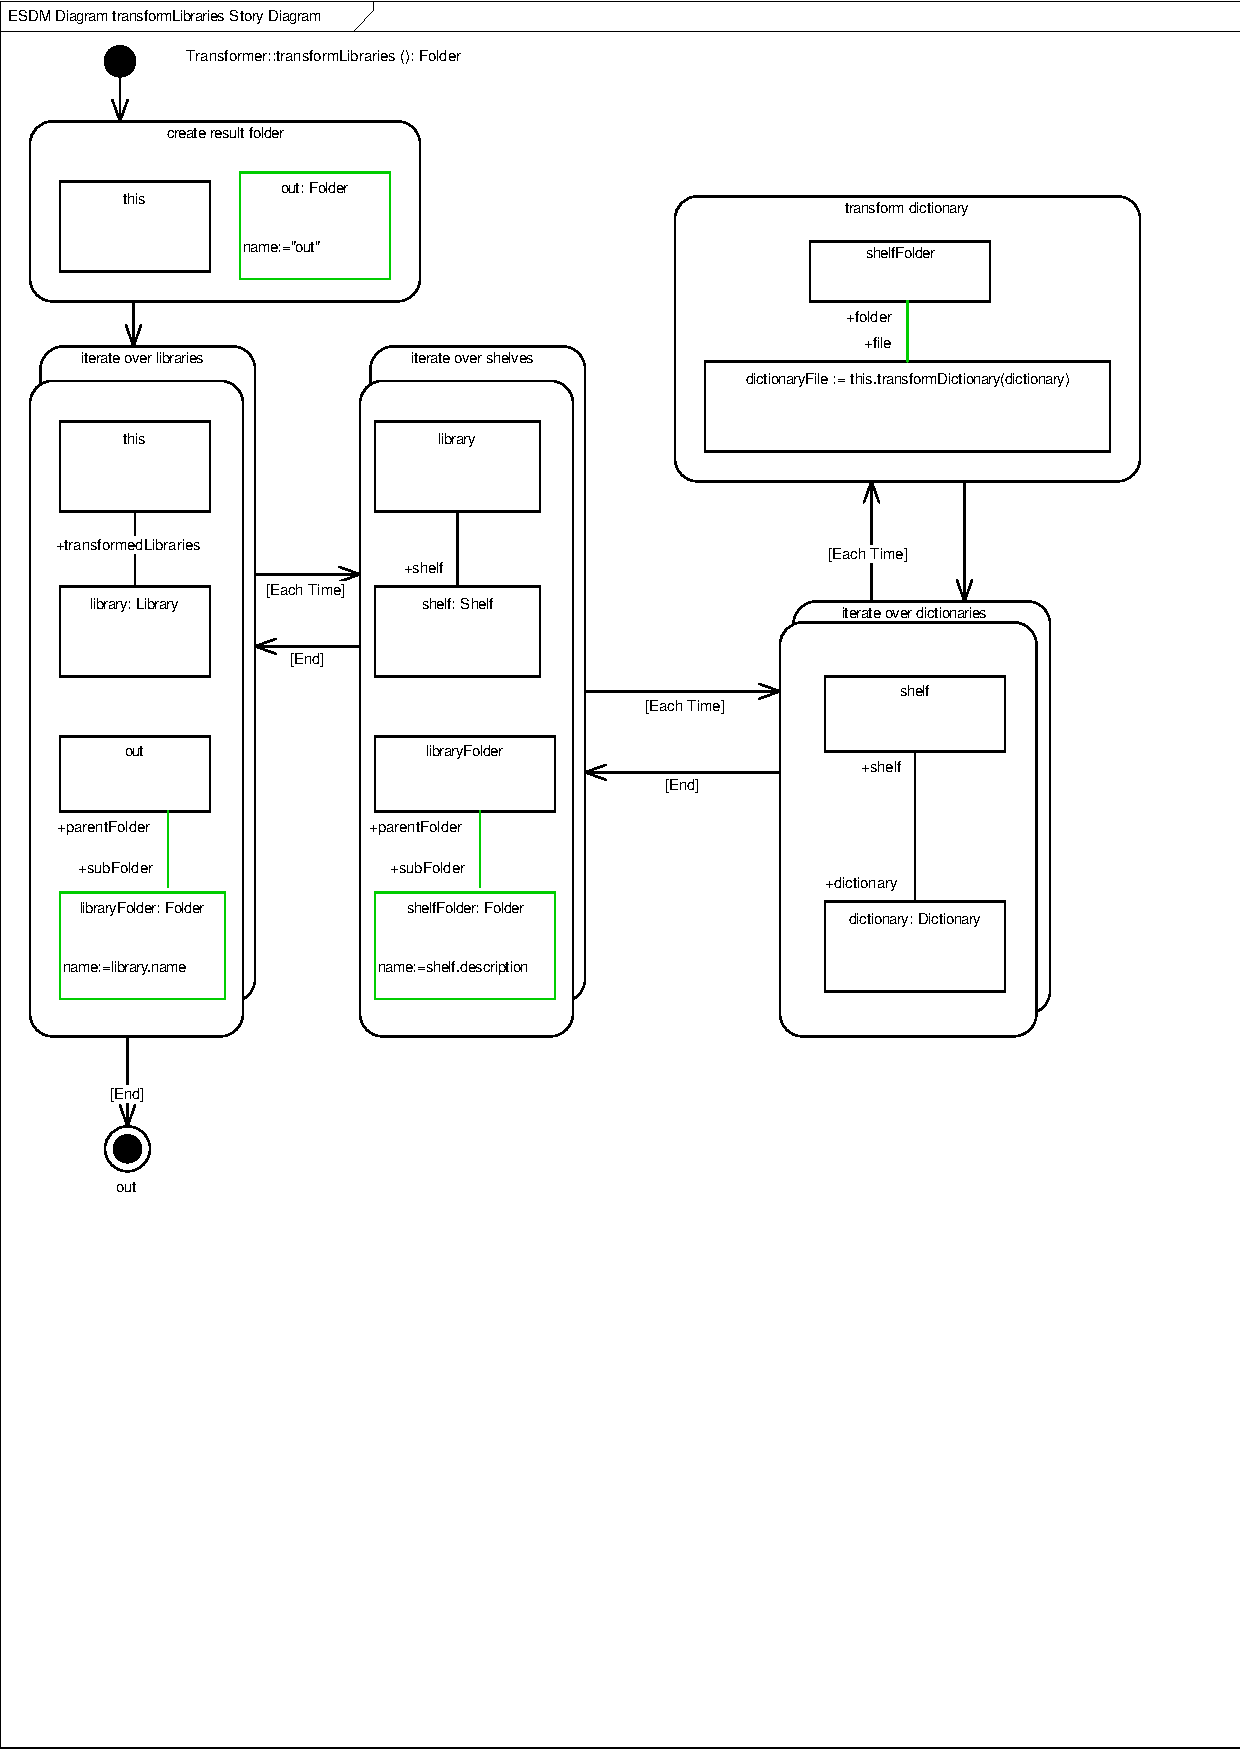
\includegraphics[width=\textwidth]{pics/moca/4ModelToMocaTree/transformLibraries}
  \caption{Iterate over all libraries, shelves and dictionaries} 
  \label{fig:moca-transformLibraries}
\end{center}
\end{figure}

\item[$\blacktriangleright$] \texttt{transformDictionary(Dictionary)~:File} (Fig.~\ref{fig:moca-transformDictionary}) does the actual work of transforming a dictionary to a file, handling authors as an optional node in the file subtree.
  %\usepackage{graphics} is needed for \includegraphics
\begin{figure}[!htbp]
\begin{center}
 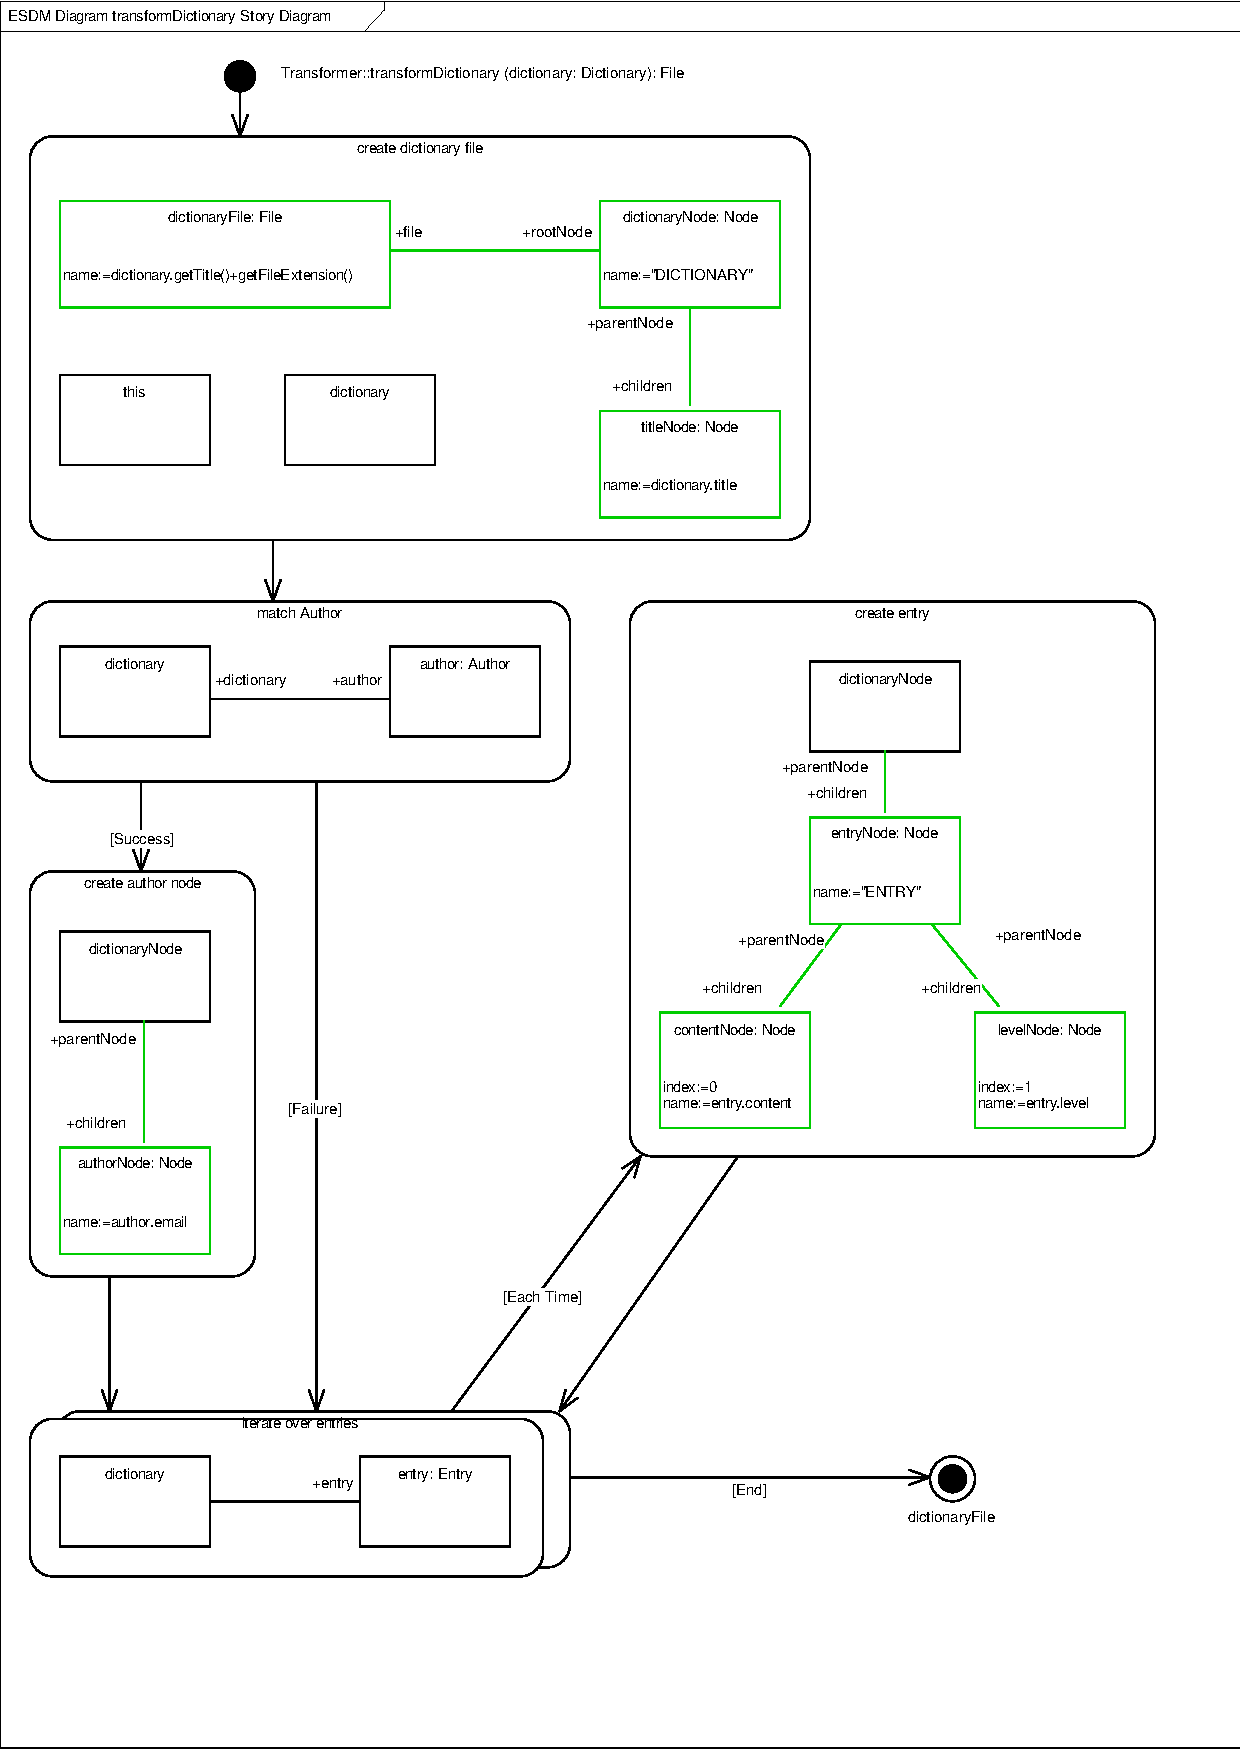
\includegraphics[width=\textwidth]{pics/moca/4ModelToMocaTree/transformDictionary}
  \caption{Create a file from a dictionary with an optional author} 
  \label{fig:moca-transformDictionary}
\end{center}
\end{figure} 
\item[$\blacktriangleright$] To invoke the model-to-tree transformation, open \texttt{MocaMain.java} (Fig.~\ref{fig:moca-8-MocaMain}) and edit lines 38-39 as follows:
\begin{verbatim}
// Perform model-to-tree transformation
transformer.setFileExtension(".dictionary");
Folder out = transformer.transformLibraries();
\end{verbatim}
The tree \texttt{out} can of course be persisted to file using \texttt{eMoflonUtil.saveModel} if you wish to inspect it before continuing.
If you did everything right, it should resemble Fig.~\ref{fig:moca-10-ParseResult2} very closely. 
\end{enumerate}